% This file was converted to LaTeX by Writer2LaTeX ver. 1.4
% see http://writer2latex.sourceforge.net for more info
\documentclass[a4paper, 12pt]{article}
\usepackage[utf8]{inputenc}
\usepackage[T1]{fontenc}
\usepackage[english]{babel}
\usepackage{amsmath}
\usepackage{amssymb,amsfonts,textcomp}
\usepackage{array}
\usepackage{hhline}
\usepackage[pdftex]{graphicx}
\usepackage{lmodern}
\usepackage[hidelinks]{hyperref} % to hide ugly links use
\def\UrlBreaks{\do\/\do-} % To break urls at the end of the line

% For bibliography:
\usepackage[
%    natbib = true,
%     backend=bibtex, % this OR biber
backend=biber,
isbn=false,
url=false,
doi=false,
eprint=false,
%    style=numeric,
%style=authoryear,
style=authoryear-comp,
sorting=ynt, % sorts names in citations by year, name, then title
sortcites = true, % to avoid first names, but check disambiguation in the very end:
uniquename=false,
uniquelist=false,
maxbibnames=3,    
maxcitenames=2 % to put "et al" after a few authors
]{biblatex}
\renewcommand*{\nameyeardelim}{\space} % to remove the coma in textcite (bug work around)
\bibliography{biblio}
% To clear the "note" field:
\AtEveryBibitem{%
	\clearfield{note}%
}
\AtEveryBibitem{%
	\clearlist{language}%
}

\emergencystretch 2em % To avoide overfull boxes
\renewcommand{\baselinestretch}{1.5}

%\topskip=40pt
%\parskip=10pt
%\parindent=0pt
%\baselineskip=15pt

\usepackage{geometry}
\geometry{a4paper, portrait, left=2.5cm, right=2.5cm}
%%\textwidth=12.978986403cm % golden ratio
%%\addtolength{\oddsidemargin}{1cm}
%%\addtolength{\evensidemargin}{1cm}
%%%\addtolength{\textwidth}{-2cm}
\addtolength{\topmargin}{-0.5cm}
\addtolength{\textheight}{1.5cm}

\title{\Huge Mate-copying in Drosophila:\\ a matter of taste or disgust?}
\author{Guillaume Lespagnol}
\date{\today}

\begin{document}
	
	\maketitle
	
	\tableofcontents
	\bigskip
%	\clearpage
	
	Examples of citation: \textcite[e.g.][118]{danchin_cultural_2018}.
	
	Or rather:
	\parencite[e.g.][118]{danchin_cultural_2018}.
	
	Or several: \textcites[e.g.][118]{danchin_cultural_2018}[but see][1789]{pike_conformist_2010}
	
	Or between brackets: \parencites[e.g.][118]{danchin_cultural_2018}[but see][1789]{pike_conformist_2010}.
	
	\parencite{framit_zotero_2019, morgan_biological_2012}.
	
	\textcite{dagaeff_drosophila_2016} demonstrated that...
	
	\section{Introduction}

	Mating matters. From sexual selection arise a variance in reproductive success between individuals that models future genotypes. This “struggle for the possession of the other sex” (Darwin, 1859) impacts the evolution in many ways, as each sex develop complex mechanisms in order to reproduce. Intersexual selection (i.e mate-choice), involves a choice from one sex and can lead to captivating and highly complex traits, such as courtships or songs in birds (Behavioral Ecology, 2008). Nevertheless, many species do not exhibit such traits and individuals must choose a mate using much more discreet signs. Since mate-choice is far to be trivial, choosing randomly and learning by trial and errors can be very expensive for naive individuals. To avoid such costs, many species have acquired the capacity to learn from the observation of others and can therefore use social learning in numerous decision-making processes.
	
	Social learning is widespread among taxa and even exists in non-social invertebrates (Coolen et al., 2005; M.E Laidre, 2010). Different mechanisms can be involved in social learning, such as teaching and copying. The simpler strategy here is to copy conspecifics. This mechanism has also been observed in several species, such as in meerkats (Thornthon \& Malapert, 2009) or in guppies, where females copy other females’ mate-choices (i.e. mate-copying) (Dugatkin \& Godin, 1992). Using others as a source of information is likely to be particularly beneficial when individual learning is costly (time consuming or dangerous), due to a cheaper, but less reliable public information (gained by observing the performance of others). Therefore, copying the mate-choice of potentially older conspecifics can be a reliable choice for naive individuals, where any mistakes can strongly reduce fitness.
	
	Mate-copying is a form of social learning in which the observation of a sexual interaction between conspecifics biases the subsequent mate-choice decision of the observer (Fish Cognition and Behavior, 2011). It has been first demonstrated in fishes (Dugatkin \& Godin, 1992), followed by observations in many vertebrates (Galef \& White, 1998; Yorzinksi \& Platt, 2010) and recently in invertebrates (Mery et al.,2009; Fowler-Finn et al., 2015). Benefits of mate-copying is double-sided, it allows naive individuals to avoid mistakes and make sure that their descendant will be preferred by conspecifics. Early studies that used species with genetic preferences of male traits showed that mate-copying can override genetic preferences (Dugatkin et al., 1996; Witte \& Ryan, 1998). By overriding genetic-based sexual preferences, mate-choice copying can have heavy evolutionary consequences that are still complex to apprehend (reviewed in Varela et al., 2018). The fact that mate-copying can shape mate-preference at population scale means that it could be at the origin of the formation of local tradition. Such traditions transmitted vertically and horizontally, for a trait-based preference and possibly for a long time can even lead to the appearance of animal culture (Brooks 1998 ; Danchin 2018).
	
	The existence of culture in non-human species has long been disputed (Laland 2013) but is increasingly accepted among scientists (Aplin et al., 2015, Whitehead 2017). The list of animals exhibiting a form of cultural tradition is growing almost every year (van Schaik et al., 2003 ; Thornton et al., 2010 ; Whiten 2017) , and one of the most recent may surprise many, Drosophila melanogaster (Danchin et al., 2018). Very few, if none, species have been studied as deeply and for whom knowledge in every scientific field (genetics, development, neuroscience…) is as extensive than Drosophila Melanogaster. Thus existence of mate-copying in this species represents a good opportunity to understand the obscure biological root of an evolutive process broadly shared in the animal kingdom.
	
	Despite a rich repertoire of different social behaviors in fly that have allowed the study of complex social processes (Pasquaretta et al., 2016; Teseo et al., 2016; Dawson et al., 2018), social learning and particularly its mechanisms are poorly understood, contrarily to non-social learning mechanisms (reviewed in Cognini et al., 2018). Yet, regarding their roles in non-social learning, two brain structures are particularly prone to be involved in mate-copying, the central complex and the mushroom body. The central complex, localized in the center of the insect brain plays a major role in decoding visual information. It receives visual inputs from the rest of the brain and controls vision-related behaviors, memory and learning (Guo et al., 2017). The mushroom body is an integrative center involved in learning, memory, decision-making and visual associative memory (Vogt et al., 2014). Concerning social learning, Monier et al. showed that dopamine and serotonin are required in mate-copying. They both are neurotransmitters driving a variety of brain function among which the formation of appetitive and aversive memory (Riemensperger et al., 2005; Sitamaran 2008; Alekseyenko et al., 2010; Berry et al., 2012; reviewed in Yamamoto et al., 2014). However, the neuronal pathways and groups of neurons involved in mate-copying are still unknown. In drosophila, depending on if the stimulus is aversive or appetitive, different groups of neurons are involved (Vogt et al., 2014 ; reviewed in Busto et al., 2010). Therefore the first step to take in order to investigate the mechanistics origin of mate-copying is to know if it involve appetitive or aversive memory.
	
	In the present study we first tested if mate-copying implies aversive or appetitive memory by isolating different kinds of stimulus contained in copulation of conspecifics. We considered that a rejection represent an aversive stimulus and acceptance of copulation an appetitive stimulus for an observer female. So, we created two treatments by presenting a male rejected by a female (``Rejection'' treatment) or a male accepted by a female (``Acceptance'' treatment), for which we measured the inclination to copy.
	
	Then we investigated deeper neuronal mechanisms of mate-copying by searching which group of neurons is required for mate-copying. By using GAL4 technology, Liu et al in 2012 have found that specific groups of neurons, localised in mushroom bodies are involved in the acquisition of aversive and appetitive olfactive memory, TH and Ddc respectively. Moreover, Vogt et al have found in 2014 that those neurons are shared by olfactive and visual memory. Given that mate-copying involves visual learning, we expected those groups of neurons to be required in its mechanisms. Also, we know that UAS-GAL4 technology can be used to block specific sets of neurons (Liu et al., 2012). Specifically, by coupling UAS-GAL4 with the Shibire protein, it is possible to temporary block specific groups of neurons labelled by GAL4, like TH and Ddc. Thus, we created two treatments (“TH” and “Ddc”), by using mutant flies expressing GAL4 in TH-labeled or Ddc-labeled neurons, for which we calculated a mate-copying score. If one group is involved in mate-copying, the corresponding treatment will exhibit a mate-copying score similar to random choice, due to the inactivation of this group.
	
	\section{Material and Methods}

	\subsection{Fly maintenance}
	
	We used the common Canton-S strain of D.melanogaster (wild-type, and UAS / Gal4 lines described above). Flies were raised and kept in 30 ml tubes containing standard corn flour-yeast-agar medium at 25° ± 1°C and 56 ± 4 \% humidity with a 12:12H light:dark cycle. Humidity and temperature were controlled and adjusted continuously with two independents automatic humidifiers and one manual heater. Medium was cooked every 3 weeks and stored at 4°C until use. Flies were manipulated with a hand-made mouth aspirator made of a glass pipette, tubing and gauze.
	
	Every morning, adult flies were removed from the breeding vials so that the newly emerged flies collected within the 6-8 hours were virgin. For Canton-S strain, 120 males and 120 females were used daily for breeding (20 tubes with 6 males and 6 females in each) and all other adults were euthanized in a freezer. For mutant strains, all adults were used for breeding. 
	
	Virgins were sexed without anesthesia, by gentle aspiration and then kept in unisex groups of 7 females or 14 males until experiments. Both demonstrator and observer flies were 3 or 4 days old. Males and females were used only once as females are reluctant to re-mate (Chapman et al., 2003) and reject males they just saw copulating (Loyau et al., 2012). After experiments, all flies were put in a food vial and cold-euthanized at the end of the day.
	
	\subsection{Fly stains and crossings}
	
	For the second experiment, we used two mutant genotypes, Ddc-GAL4/w+;;UAS-Shits/+ and w+/w-;;UAS-Shits/TH-GAL4 ,obtained by crossing homozygous lines. 
	
	UAS-Shits is a transgene that contains an GAL4-specific enhancer,UAS (Upstream Activating Sequence) driving the production of Shibire protein in cells where GAL4 is present. Shibire is a thermosensitive protein that inhibit neuronal activity at restrictive temperature (30°C) by preventing vesicle recycling (Kitamoto 2001). Ddc-GAL4 and TH-GAL4 drive production of a transcriptional activator (GAL4) only in specific subsets of dopaminergic neurons. GAL4 activates the expression of genes downstream to UAS. Ddc-GAL4 labels neurons involved in appetitive olfactory memory (reference):the blockade of these neurons by Shibire protein has been shown to impair the acquisition of such memory at restrictive temperature.TH-GAL4 labels neurons involved in aversive olfactory memory (Liu et al., 2012).
	
	As white recessive mutation w- impairs fly vision (Götz 1968), we used mutant females with one wild-type copy of the white gene for the experiments. To do so, we crossed w+;;Shits males with females from each Gal4 line. To obtain w+;;Shits strain from a w-;;Shits strain, we crossed males w-;;Shits with females w+;;TM2/TM6b over two generations and selected TM2 non TM6B flies only, with CO2 anesthesia, and we then isolated homozygous w+;;Shits progeny.
	
	TH-GAL4 and Ddc-GAL4 lines were provided by Guillaume Isabel in the same Canton-S background as the Wild-type strain.
	
	\section{General experimental procedures}
	
	Artificial male phenotypes were created by dusting virgin males with pink or green powder (Mery et al., 2009). Each vial of males was randomly assigned to a color. Before the experiment started, males were placed in a clean vial to remove the excess of dust for at least 20-30 min. Experiments took place in the same tube set-up and a similar but slightly modified speed-learning protocol than described in Dagaeff et al. 2016 (Figure 1, see also specific experiment section).
	
	Demonstrator and observer flies were placed in two compartments of double plastic tubes, separated by a thin glass partition and closed by cotton plugs. All replicates were run in blocks of six trials with cardboard barriers between experimental set-ups, to prevent information exchange between the flies and disturbance from the surroundings. 
	
	During the demonstration, we always showed two different male phenotypes (color) to the observer females, with one favorite that copulated with the demonstrator female. If demonstrator females refused to copulate, the trial was discarded. Specifics of demonstrations for each experiment are described above (see specific experiment section).
	
	Once the demonstrations were over, we started the mate-copying test by introducing a couple of colored virgin males (one of each color) in front of the observer female and we removed the partition, allowing the female to freely choose between males for 30 min. The partition was put back in place when all three flies were in the same side of the tubes, to promote proximity between flies. During that time, we recorded the time of first courtship for each male, the time when copulation started and the color of the chosen male. The onset of the courtship was defined as the first wing-extension of a male (Figure 2).

	\begin{figure}
		\centering
		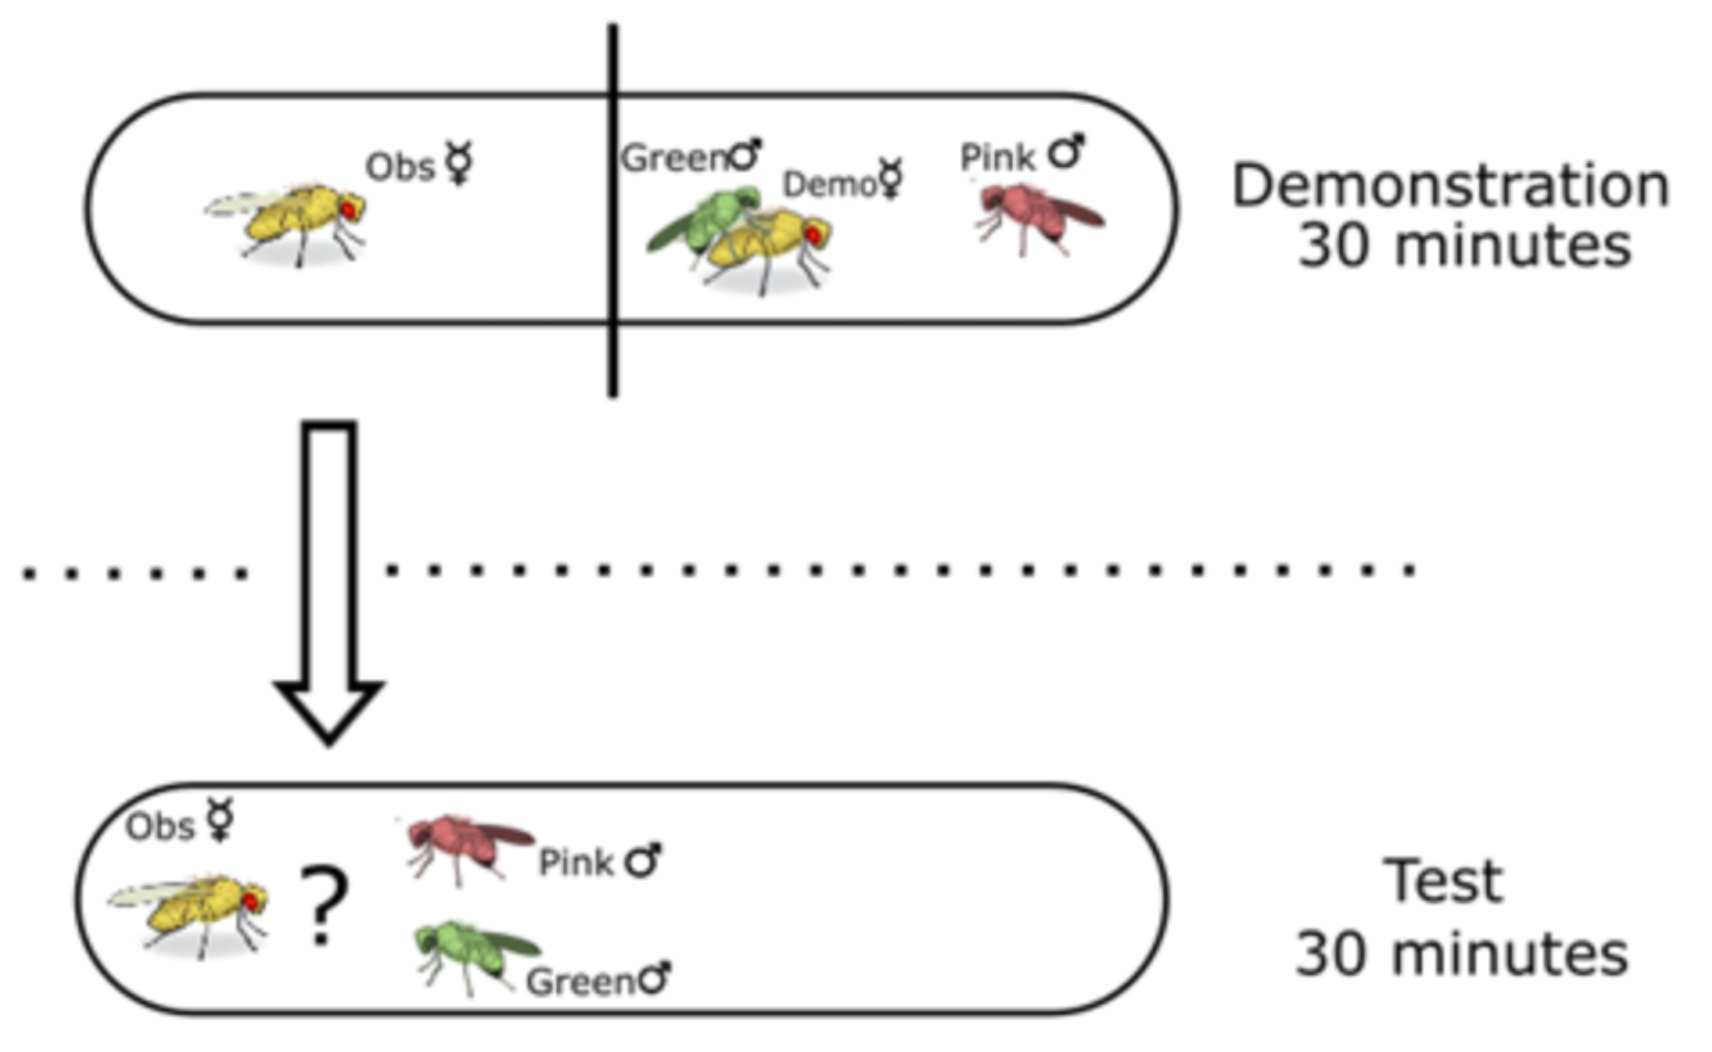
\includegraphics[width=0.8\textwidth]{images/tubes-nolegend.png}
		\caption{Écrire la légende ici.}
	\end{figure}

	\subsection{Acceptance/Rejection experiment}
	
	During this first experiment, we tested whether mate-copying is achieved through aversive or appetitive memory. To do so, we split the negative and positive information given by the usual mate-copying demonstration. A classical demonstration, in which a demonstrator female chooses between two males, contains a rejection (negative information) of a male and an acceptance (positive information) of the other one. We thus created three demonstration treatments: (1) a control where a demonstrator female freely chooses between two males, (2) an “acceptance” treatment with one accepted male copulating with a demonstrator female, and (3) a rejection treatment with one male actively rejected by a female (Figure 3).
	
	\subsection{Neuronal blockade experiment}
	
	This second experiment aimed at exploring the mechanisms underlying the results of the Acceptance/Rejection experiment by discovering one group of dopaminergic neurons involved in mate-copying.
	
	The demonstration was similar to classical protocol (Figure 1), but we used Ddc-GAL4/w+;;UAS-Shits/+ (treatment “Ddc”) and w+/w-;;UAS-Shits/TH-GAL4 mutants (treatment “Gal4”) as observer females. The use of these mutants allowed us to have a temporal control on specific sets of neurons presumably involved in appetitive (Ddc) or aversive (TH) memory, thanks to the thermosensitive activation of Shibire. During the demonstration and 30 minutes before, observer mutant females were heated to a restrictive temperature of 33°C, thanks to a heating mat under the tube of these females. At 33°C, Shibire protein blocks the neurons in which it is expressed, and thus the acquisition of appetitive memory should be blocked in observer females of “Ddc” treatment, and the acquisition of aversive memory in “TH” females. 
	
	After all copulations ended, demonstrator males and females were removed. Observer females were then stored individually in clean tubes at 25°C for 3-4 hours to ensure that labelled neurons are no more blocked, then we proceeded to a classical test at 25°C.

	\begin{figure}
%		[Warning: Draw object ignored]
		\caption{Ré-exporter le draw ici.}
	\end{figure}

	\subsection{Mate-copying score}

	As in previous studies (Danchin et al., 2018; Nöbel et al., 2018; Monier et al., 2018), a mate-copying score evaluated female’s tendency to copy the choice of the demonstrator. A mate-copying score of 1 was assigned to females that copulated with the color preferred by demonstrator females and a score of 0 in the opposite case. For each treatment, a mate-copying index was calculated as the mean of mate-copying scores per treatment, a random choice indicated by a value of 0.5. All replicates where only one male courted the female before copulation were discarded because in these situations the female was not unambiguously in a position to make a choice between the two colors.

	\subsection{Statistical analyses}

	All statistical analyses were performed with the R software version 3.5.1 (R Core Team, 2018).
	For each treatment, the difference from a random choice was tested with a binomial test. Mate-copying scores were then analyzed in a generalized linear mixed model (GLMM, package lme4 (Bates et al., 2015)). Starting models contained the following fixed effects: treatment, normalized air pressure (air pressure in Toulouse-Blagnac weather station, at the time of the beginning of the experiment, minus mean air pressure), normalized air pressure variation within the six preceding hours and all interaction between these three variables, experimenter effect and its interaction with treatment. A random “block” effect was also introduced in the models to account for the non-independence of observer flies from the same block of 6 tubes-set up trained and tested in parallel. The significance of fixed effects was tested using Wald chi-square tests included in ANOVA function (car package, Fox and Weisberg 2011). Model simplification was achieved by successive withdrawal of the non-significant terms in a backward selection approach, using P-values and starting with the highest-order interaction. The final model was chosen as the one with the lowest Akaike Information Criteria (AIC, Akaike, 1969). Comparisons between treatments were done using post-hoc X² tests. 

	\subsection{Ethical statements}

	Behavioral observations of D. melanogaster required no ethical approval and complied with French laws regarding animal welfare. We kept the number of flies used in this study as small as possible. We handled flies by gentle aspiration without anesthesia to minimize damage and discomfort. After the experiments, individuals were euthanized in a freezer at -20°C.

	\section{Results}

	\subsection{A/R Experiment}
	\label{subsec:AR-experiment}

	In total, we tested 850 females among which 530 copulated, including 192 with double-courtship, 64 for each treatment. First we tested for female's color preference with binomial test but neither in the demonstration (N = 850, 426 females copulated with green males and 424 copulated with pink males; binomial test: P = 0.973) nor the test (N = 192, 90 copulated with pink and 102 with green males; binomial test: P = 0.427) was there any significant difference between the two colors.

	For each treatment, the difference from random choice was tested with a binomial test, acceptance (where the observer female sees a copulation, N = 64, P {\textless} 0.001) and control (N = 64, P = 0.03) were both significantly different from random, but rejection treatment (where the observer female sees a male rejected without copulation, N = 64, P = 0.382) was not (Figure 4).

	To test for the significance of mate copying among treatments, we built a global model including the effects of experimenter, treatment, normalized air pressure (actual air pressure minus global mean of air pressure), normalized air pressure variation (for the last six hours) and the interaction between air pressure and variation of air pressure. Only the treatment had a significant effect on mate-copying (GLMM, $\chi^2$: $N = 192$, $\chi^2 = 10.447$, $p = 0.005$), air pressure (GLMM, $\chi $²: N = 192, $\chi $² = 0.572, P = 0.449) and variation of air pressure (GLMM $\chi $²: N = 192, $\chi $² = 1.831, P = 0.176) were non-significant. The interaction between air pressure and variation of air pressure was close to be significant (GLMM $\chi $²: N = 192, $\chi $² = 2.946, P = 0.086), as we could have expected in regard of the results of Dagaeff et al., 2016. No significant difference has been found between control and acceptance treatments ($\chi $² = 1.76, P = 0.18; Fig4), but both are different from rejection treatment (acceptance - rejection: $\chi $² = 11.62, P {\textless} 0.005; control - rejection: $\chi $² = 4.52, P = 0.033; Fig4).
	
	Voir Figure~(\ref{fig:histogramme-mcs}).

	\begin{figure}
		\centering
		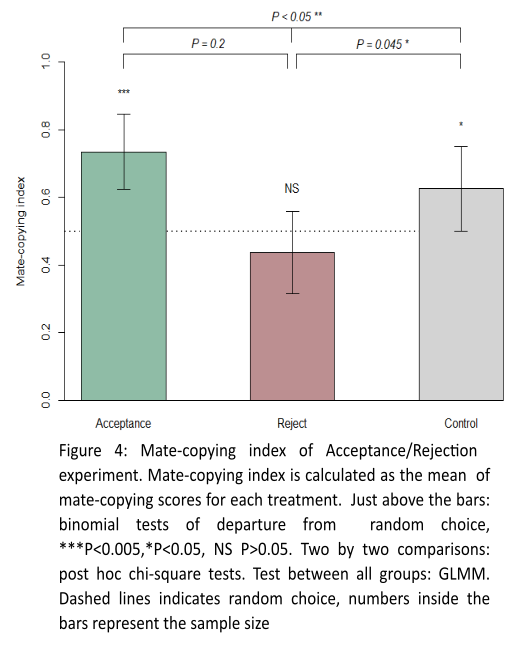
\includegraphics[width=0.8\textwidth]{images/histogramme-mcs}
		\caption{Légende ici.}
		\label{fig:histogramme-mcs}
	\end{figure}



\clearpage
\newrefcontext[sorting=nyt] % sorts the bibliography by name first, then year, title
\printbibliography

\end{document}
